% figures/counterexample.tex

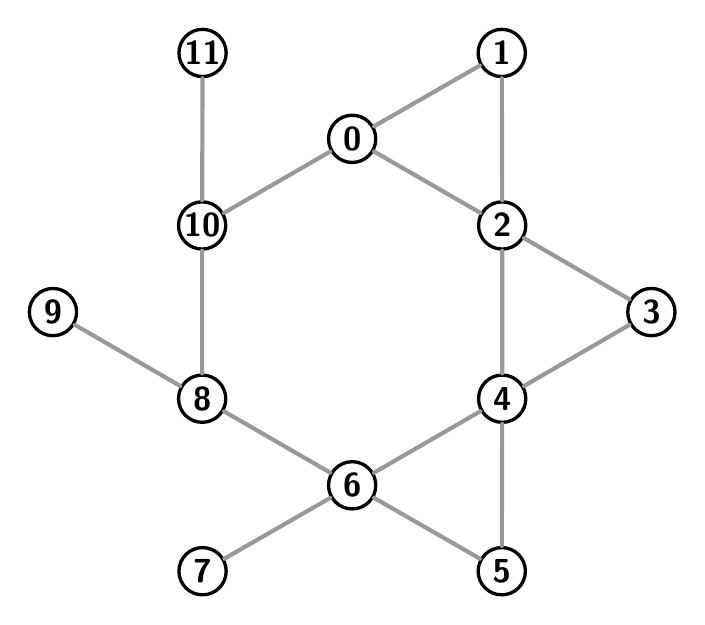
\begin{tikzpicture}[
    % Define the style for the vertices
    vNode/.style={
        circle, 
        draw=black, 
        fill=white, 
        very thick, 
        inner sep=0pt, 
        minimum size=6mm
    },
    % Define the style for the labels inside or near nodes
    vLabel/.style={
        font=\sffamily\bfseries\large
    },
    % Define the style for the connections
    edgeStyle/.style={
        draw=gray!80, 
        line width=1.5pt, 
        line cap=round
    }
]

    % --- COORDINATE DEFINITIONS ---
    % Central Hexagon Radius
    \def\hexR{2.2} 
    % Outer Nodes Radius
    \def\outR{3.8}

    % --- NODES ---
    % Inner Hexagon Nodes (0, 2, 4, 6, 8, 10)
    % Placed at 60-degree increments starting from 90 to keep it upright
    \foreach \i/\name in {0/0, 1/2, 2/4, 3/6, 4/8, 5/10} {
        \node[vNode] (V\name) at ({90 - \i*60}:\hexR) {};
        \node[vLabel] at (V\name) {\name};
    }

    % Outer Nodes (1, 3, 5, 7, 9, 11)
    % Placed between the inner nodes for symmetry
    \foreach \i/\name in {0/1, 1/3, 2/5, 3/7, 4/9, 5/11} {
        \node[vNode] (V\name) at ({60 - \i*60}:\outR) {};
        \node[vLabel] at (V\name) {\name};
    }

    % --- EDGES ---
    % Hexagon Ring
    \draw[edgeStyle] (V0) -- (V2) -- (V4) -- (V6) -- (V8) -- (V10) -- (V0);

    % Top Triangle (0-1-2)
    \draw[edgeStyle] (V1) -- (V0);
    \draw[edgeStyle] (V1) -- (V2);

    % Right Triangle (2-3-4)
    \draw[edgeStyle] (V3) -- (V2);
    \draw[edgeStyle] (V3) -- (V4);

    % Bottom Right Triangle (4-5-6)
    \draw[edgeStyle] (V5) -- (V4);
    \draw[edgeStyle] (V5) -- (V6);

    % The "Hanging" Edges (7, 9, 11)
    \draw[edgeStyle] (V7) -- (V6);
    \draw[edgeStyle] (V9) -- (V8);
    \draw[edgeStyle] (V11) -- (V10);

\end{tikzpicture}